\section{Methodology}
\label{sec:methodology}

This chapter describes the systematic literature review process used to
assemble the evidence base for the gap analysis presented in
Section~\ref{sec:synthesis_gap}. It covers the governing review framework
and search strategy, the seed paper and corpus design, the citation
snowballing and screening procedure, and the resulting bibliometric profile
of the final reading list. The PRISMA 2020 flow diagram
(Figure~\ref{fig:prisma}) summarises how the corpus was reduced
from initial retrieval to the 123-paper final reading list referenced
throughout the review.

\subsection{Review Design and Governing Framework}
\label{sec:methodology:framework}

This study adopts a Systematic Literature Review (SLR) methodology, defined as a
comprehensive, pre-planned strategy for identifying, critically appraising, and synthesising
research relevant to a clearly stated research question \citep{KitchenhamCharters2007}.
The review follows the \textbf{PRISMA 2020} reporting guidelines \citep{Page2021}, which
organise the review process into four stages: \textit{Identification}, \textit{Screening},
\textit{Eligibility}, and \textit{Inclusion}. The eight-step systematic review process of
\citet{XiaoWatson2019} guided the overall research design, from problem formulation
through synthesis, and the snowballing procedure of \citet{Wohlin2014} was used for
forward and backward citation search.


The review addresses the following operational question:
\begin{quote}
\textit{What methods have been proposed for decentralised, adapter-based multi-task inference over a shared frozen transformer backbone, and what are the open research gaps?}
\end{quote}
\begin{quote}
\textit{This operational question is the literature-searchable form of a broader feasibility question: whether the existing literature provides sufficient building blocks for lightweight task-specific adapters to be discovered, retrieved, composed, and served across a peer-to-peer network of nodes sharing a single frozen transformer backbone, without centralised orchestration — and if not, where the gaps lie.}
\end{quote}


The review synthesises three intersecting fields: (i)~parameter-efficient fine-tuning
(PEFT) and adapter architectures; (ii)~distributed and peer-to-peer (P2P) machine learning
systems; and (iii)~multi-task large language model (LLM) serving and inference. This
three-pillar framing directly determined the corpus design: Groups G1--G2 cover PEFT
methods and adapter composition; Groups G3 and G6 cover decentralised and federated
learning; Groups G4--G5 cover inference systems and mixture-of-experts (MoE) routing. The
review was structured concept-centrically following \citet{Webster2002}, with each
synthesis chapter addressing one or two thematic groups.

\subsection{Relationship to Prior Reviews}
\label{sec:methodology:prior_reviews}

A key methodological requirement of any SLR is to establish that no equivalent review 
already exists \citep{KitchenhamCharters2007}. The closest existing works each 
cover one or at most two of the three pillars examined here: parameter-efficient fine-tuning, 
peer-to-peer or federated machine learning, and multi-tenant LLM inference serving. 
\citet{Han2024} and \citet{DingNature2023} provide comprehensive surveys of PEFT methods 
but do not address distributed or P2P deployment. \citet{Sajina2021} examines P2P 
deep learning architectures but predates the PEFT-at-scale era and does not address 
adapter-level exchange. \citet{WangAIReview2024} surveys PEFT methodologies without 
a systems or decentralisation dimension. To the best of the author's knowledge, no prior review comprehensively synthesises PEFT, P2P systems, and multi-tenant serving at the architectural level, suggesting that this intersection remains unaddressed.

\subsection{Seed Paper Selection}
\label{sec:methodology:seeds}

The search was anchored on eight foundational seed papers (Group G0), selected on three
criteria: (i)~direct relevance to at least two of the three core themes; (ii)~citation
impact of at least 300 citations at the time of selection; and (iii)~publication in a
top-tier venue (ICML, ICLR, NeurIPS, ACL/EMNLP/EACL, MLSys, or a Scopus Q1 journal).
These seeds span the three pillars of the review: adapter architectures
\citep{Houlsby2019, Hu2022, Pfeiffer2020hub, Pfeiffer2021fusion}, multi-task P2P learning
\citep{Sajina2024}, distributed LLM inference \citep{Borzunov2023}, PEFT surveys
\citep{Han2024}, and multi-tenant adapter serving \citep{Sheng2024}.

\subsection{Pre-Validated Corpora (G1--G6)}
\label{sec:methodology:corpora}

In parallel with snowballing, six thematically focused pre-validated corpora (Groups
G1--G6) were assembled through targeted curation of leading publication venues. Undermind,
an AI-assisted academic search tool, was used to accelerate retrieval of candidate papers
from ACL, EMNLP, NeurIPS, ICML, MLSys, and related venues for each of the six groups.
The Undermind queries are reproduced verbatim in Appendix~A. All inclusion decisions
remained with the human reviewer: Undermind accelerated retrieval of candidates, but
relevance assessment and selection were performed manually. Table~\ref{tab:groups} summarises
the six groups, their thematic scope, and their contribution to the final reading list.

\begin{table}[H]
\centering
\caption{Pre-validated corpus groups: scope, size, and review section coverage.}
\label{tab:groups}
\begin{tabular}{lp{5cm}rrl}
\toprule
\textbf{Group} & \textbf{Theme} & \textbf{\textit{n} pre-val.} & \textbf{\textit{n} final} & \textbf{Section(s)} \\
\midrule
G0 & Foundational seeds (PEFT, P2P, serving) & 8   & 20  & \ref{sec:peft}--\ref{sec:adapter_composition}, \ref{sec:inference_systems} \\
G1 & PEFT methods beyond adapters and LoRA   & 59  & 12  & \ref{sec:peft} \\
G2 & Adapter composition for multi-task NLP  & 37  & 15  & \ref{sec:adapter_composition} \\
G3 & Decentralised and P2P ML systems        & 95  & 11  & \ref{sec:p2p_federated} \\
G4 & Adapter multiplexing for LLM inference  & 51  & 12  & \ref{sec:inference_systems} \\
G5 & Routing and MoE for modular PEFT        & 35  & 9   & \ref{sec:moe_routing} \\
G6 & Federated PEFT for transformer NLP      & 66  & 29  & \ref{sec:p2p_federated} \\
Other & Manual additions (Scopus/WoS forward snowball) & --- & 15 & cross-cutting \\
\midrule
\textbf{Total} & & \textbf{351} & \textbf{123} & \\
\bottomrule
\end{tabular}
\end{table}

Because G1--G6 papers were assembled through targeted manual curation, they bypassed both
the year filter and the automated domain-relevance filter applied to snowballed candidates.
Pre-2021 foundational works (e.g., Houlsby et al. 2019, Hu et al. 2022) entered via this
route. The year 2021 was adopted as the lower bound for snowballed records because the
confluence of LoRA \citep{Hu2022} and widespread large-scale transformer deployment marks
the practical onset of the PEFT-at-scale era addressed by this review.

\subsection{Citation Snowballing}
\label{sec:methodology:snowballing}

Forward and backward citation snowballing was conducted on the G0 seeds following the
procedure of \citet{Wohlin2014}. Backward snowballing examined the reference lists of each
seed; forward snowballing identified subsequent works citing the seeds. One wave of
snowballing was executed; saturation was assessed by inspecting the overlap between newly
retrieved candidates and the pre-validated G1--G6 corpora, with high overlap indicating
diminishing marginal returns.

Snowballing was executed programmatically via the \textbf{Semantic Scholar Academic Graph
API} \citep{SemanticScholar2023}, supplemented by the Scopus (Elsevier) and ACL Anthology
engines. The Web of Science Starter API was used in a post-hoc enrichment role, appending
WoS accession numbers and citation counts to already-retrieved records, not as a source of
new candidates. The search was executed on \textbf{2026-04-21}. In total, 1,150 raw
records were retrieved; after deduplication by DOI and Semantic Scholar paper identifier,
\textbf{972 unique records} entered the title screening stage (178 duplicates removed).

\subsection{Inclusion and Exclusion Criteria}
\label{sec:methodology:criteria}

Records were assessed against the pre-defined criteria in
Table~\ref{tab:ie_criteria}, applied consistently across all screening stages.

\begin{table}[H]
\centering
\caption{Inclusion and exclusion criteria applied across all screening stages.}
\label{tab:ie_criteria}
\small
\setlength{\tabcolsep}{3pt}
\begin{tabularx}{\textwidth}{p{1.9cm}XX}
\toprule
\textbf{Criterion} & \textbf{Inclusion} & \textbf{Exclusion} \\
\midrule
Publication year &
  $\geq$ 2021 (snowballed records); pre-2021 foundational works via G0--G6 &
  $<$ 2021 for snowballed records \\
Language &
  English (implicit --- source databases index predominantly English-language works) &
  Non-English works not surfaced by the APIs \\
Document type &
  Peer-reviewed conference paper, journal article, or arXiv preprint subsequently cited in at least one peer-reviewed work within the corpus &
  Blog posts, grey literature, software documentation, workshop papers without proceedings \\
Topical relevance &
  Addresses $\geq$1 of: (a) PEFT/adapters; (b) distributed/P2P/federated ML; (c) multi-task LLM serving &
  Exclusively covers unrelated domains (CV, audio, RL) with no NLP or systems angle \\
Abstract availability &
  Accessible via API or pre-validated corpus &
  No accessible metadata and no resolvable DOI \\
\bottomrule
\end{tabularx}
\end{table}

The arXiv inclusion threshold serves as a minimal proxy for community engagement: a preprint cited by at least one peer-reviewed work in the corpus has demonstrably influenced the reviewed literature. The threshold was set conservatively low to favour recall, as recent preprints (2025--2026) may not yet have accumulated peer-reviewed citations. The implications of this criterion for corpus composition are discussed in Section~\ref{sec:conclusion:threats}.



\subsection{Screening Procedure}
\label{sec:methodology:screening}

Title screening was applied to all 972 snowballed records in three layers.
\textbf{Layer~1} excluded records published before 2021 based on publication year metadata.
\textbf{Layer~2} scored each title against four pre-defined term sets --- \textit{PEFT/adapters},
\textit{LLM/transformers}, \textit{systems/serving}, and
\textit{distributed/P2P/federated} --- using exact substring matching (term-set version~1.0).
Records matching $\geq$2 term sets were flagged for inclusion; records matching exactly one
non-LLM term set were queued for triage; LLM-only matches and zero-match records were
excluded. The author verified all keyword-flagged records during the subsequent review stages.
\textbf{Layer~3} resolved the remaining 130-record triage queue through manual assessment
of title and venue metadata. The author reviewed all 130 records individually; to support
consistency across this batch, an automated classifier generated preliminary sorting
suggestions, which the author independently verified before finalising each classification.
Records classified as UNCERTAIN (19 of 130) were retained for closer inspection. The
classifier model identifier and per-record decisions are recorded in the audit log.
Table~\ref{tab:screening} shows the screening outcomes.

\begin{table}[H]
\centering
\caption{Title screening outcomes across the 972 snowballed records.}
\label{tab:screening}
\begin{tabular}{lr}
\toprule
\textbf{Decision} & \textbf{\textit{N}} \\
\midrule
INCLUDE (keyword-matched, Layer~2)     & 162 \\
Promoted to INCLUDE (Layer~3 triage)  &  51 \\
UNCERTAIN --- retained for manual inspection &  19 \\
EXCLUDE (Layer~2 + Layer~3 confirmed)  & 740 \\
\midrule
\textbf{Total screened}                & \textbf{972} \\
\bottomrule
\end{tabular}
\end{table}

The automated classifier operated exclusively at the title level, processing 
title and venue name only; no abstracts or full-text content were submitted 
to the model. All final inclusion and exclusion decisions were made by the author. 
The model identifier, term-set version, and per-record decisions are recorded 
in the audit log (\texttt{log\_screening\_2026-04-21.json}).

\subsection{Enrichment and Tier Classification}
\label{sec:methodology:enrichment}

All records passing title screening were merged with the 352-paper pre-validated corpus
(G0--G6) and enriched with full abstracts and keyword metadata via the Semantic Scholar
batch API and OpenAlex. A topical-relevance filter subsequently removed off-topic records
(6 excluded) and deprioritised low-citation arXiv preprints lacking a Tier~1 topic signal
(32 moved to a rescue file). The remaining \textbf{464 records} were classified into three
tiers based on combined title, abstract, and keyword signal:

\begin{table}[H]
\centering
\caption{Tier classification of the 464-paper enriched corpus.}
\label{tab:tiers}
\begin{tabular}{llrr}
\toprule
\textbf{Tier} & \textbf{Criteria} & \textbf{\textit{N}} & \textbf{\%} \\
\midrule
Tier~1 & PEFT + distributed/P2P + LLM (all three) &  90 & 19.4 \\
Tier~2 & Two of the three themes                  & 141 & 30.4 \\
Tier~3 & Foundational or tangential (one theme)   & 233 & 50.2 \\
\midrule
\textbf{Total} & & \textbf{464} & \\
\bottomrule
\end{tabular}
\end{table}

\begin{figure}[H]
  \centering
  
\includegraphics[width=1\linewidth]{fig_slr6_tier_breakdown.pdf}
  \caption{Tier breakdown of the 464-paper relevant corpus.
           Tier~1 papers (90, 19.4\%) address all three themes;
           Tier~2 (141, 30.4\%) address two;
           Tier~3 (233, 50.2\%) address one theme.}
  \label{fig:tiers}
\end{figure}

As Figure~\ref{fig:tiers} shows, the majority of the corpus falls into Tier~2 
and Tier~3, with Tier~1 papers representing the narrowest intersection of all three themes.
Tiers served as a reading-priority guide following the three-pass method of
\citet{Keshav2007}: Tier~1 papers received full reads, Tier~2 selective reads, and Tier~3
abstract-level assessment. Venue quality of the 464-paper corpus: 166 papers (35.8\%) were
published in CORE A$^*$ or Scopus Q1 venues; 189 (40.7\%) in other peer-reviewed
conferences or journals; 91 (19.6\%) were arXiv preprints without a published venue; and
18 (3.9\%) had unknown or missing venue metadata.

\subsection{Bibliometric Overview}
\label{sec:methodology:bibliometric}

The final corpus of 123 papers spans the period 2002--2026, with a marked concentration
in the 2021--2025 window (107 papers, 87\% of the corpus). The most active year is 2024 with
38 papers (31\% of total), followed by 2025 with 20 (16\%) and 2023 with 19 (15\%),
confirming that the field is both active and growing. Publication volume accelerates
sharply after 2022, coinciding with the proliferation of LoRA-based PEFT papers and
adapter-serving systems.

\begin{table}[H]
\centering
\caption{Publication year distribution of the 123-paper reviewed corpus.}
\label{tab:year_dist}
\begin{tabular}{lrr}
\toprule
\textbf{Year} & \textbf{Papers} & \textbf{\% of corpus} \\
\midrule
2002 & 1 & 0.8 \\
2011 & 1 & 0.8 \\
2016 & 1 & 0.8 \\
2017 & 1 & 0.8 \\
2019 & 4 & 3.3 \\
2020 & 5 & 4.1 \\
2021 & 17 & 13.8 \\
2022 & 13 & 10.6 \\
2023 & 19 & 15.4 \\
2024 & 38 & 30.9 \\
2025 & 20 & 16.3 \\
2026 & 3 & 2.4 \\
\midrule
\textbf{Total} & \textbf{123} & \textbf{100} \\
\bottomrule
\end{tabular}
\end{table}

Figure~\ref{fig:venues} presents the venue distribution 
of the enriched corpus, confirming the dominance of ACL and EMNLP 
as the primary publication outlets. Conference and journal proceedings dominate the corpus, with the most frequent venues being ACL/EMNLP (25 papers combined), ArXiv preprints (9 papers), NeurIPS/NeurIPS-style (8 papers), and ICML/MLSys (7 papers combined). Figure~\ref{fig:bibliometric} presents
the year distribution visually. 

\begin{figure}[H]
  \centering
  
\includegraphics[width=1\linewidth]{fig_slr5_venues.pdf}
  \caption{Venue distribution of the 464-paper enriched corpus.
           ACL/EMNLP comprises the largest venue category (25 papers),
           followed by arXiv preprints (9), NeurIPS (8), and ICML/MLSys (7).}
  \label{fig:venues}
\end{figure}

The most densely covered concept-matrix dimension is \textbf{adapter exchange} (present in
the majority of the 123 papers), while \textbf{peer-to-peer topology} and
\textbf{discovery mechanism} remain the least covered dimensions, directly motivating
the gaps identified in Section~\ref{sec:synthesis_gap}.

\begin{figure}[H]
  \centering
  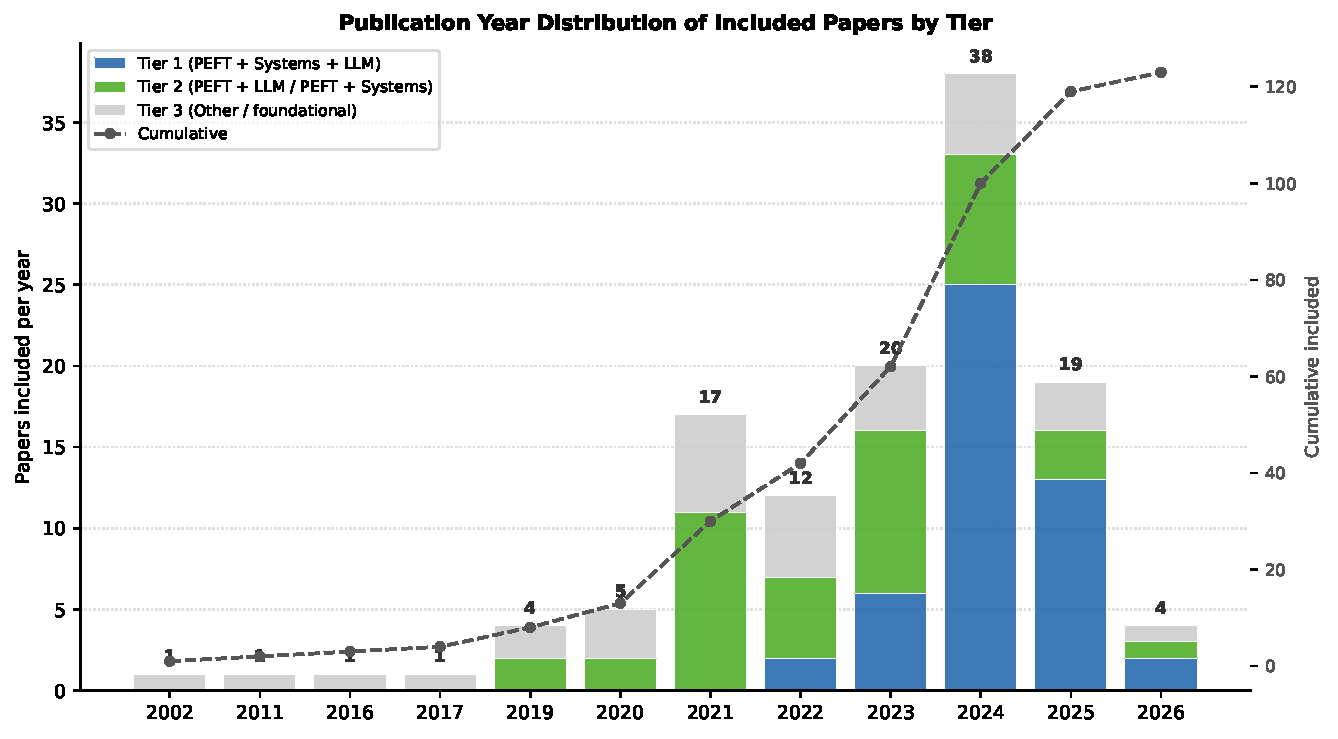
\includegraphics[width=1\linewidth]{figures/fig_slr3_year_distribution.pdf}
  \caption{Year distribution of the 123-paper reviewed corpus,
           showing the acceleration of publication volume from 2023 onward.}
  \label{fig:bibliometric}
\end{figure}

\subsection{Abstract-Level Review}
\label{sec:methodology:abstract}

Following \citet{Keshav2007}, the author conducted an abstract-level review across all 552 records
(464 enriched corpus records after rescues were resolved, plus 88 records from forward
citation snowballing on Scopus and WoS that were title-screened and added to the review). To support
decision consistency across a corpus of this size, each abstract was accompanied by an automated
advisory note providing a one-sentence summary, a relevance assessment relative to the three core
themes, and a preliminary KEEP / SKIP / DEFER recommendation. These notes served as a consistency
aid; all final decisions were made by the author after independent assessment. The model identifier, the automated suggestion,
and the author's final decision are logged per record in
\texttt{S7b\_abstract\_reviewed\_final.csv} to support reproducibility checks.

\begin{table}[H]
\centering
\caption{Abstract review outcomes (552 records reviewed).}
\label{tab:abstract}
\begin{tabular}{lrr}
\toprule
\textbf{Decision} & \textbf{\textit{N}} & \textbf{\%} \\
\midrule
KEEP (included in Zotero corpus)     & 214 & 38.8 \\
SKIP (excluded after abstract)       & 338 & 61.2 \\
DEFER (requires closer reading)      &   0 &  0.0 \\
\midrule
\textbf{Total reviewed}              & \textbf{552} & \\
\bottomrule
\end{tabular}
\end{table}

KEEP papers were exported to Zotero for full-text reading via RIS format\\
(\texttt{08\_zotero\_ready\_2026-05-02.ris}). Following full-text assessment and quality
review, \textbf{123 papers} were confirmed for inclusion in the final reading list\\
(\texttt{13\_final\_reading\_list\_2026-05-12.csv}), representing the evidentiary base
for this review.

Figure~\ref{fig:prisma} presents the complete PRISMA 2020 flow diagram \citep{Page2021}, tracing all records from initial retrieval to final inclusion. The largest reduction occurs at the title screening stage, where 791 of 972 deduplicated records (81\%) were excluded, primarily for predating 2021 or failing the keyword-based relevance filters --- reflecting a deliberately broad initial retrieval strategy designed to favour recall before the more selective abstract and full-text stages.

\begin{figure}[H]
  \centering
  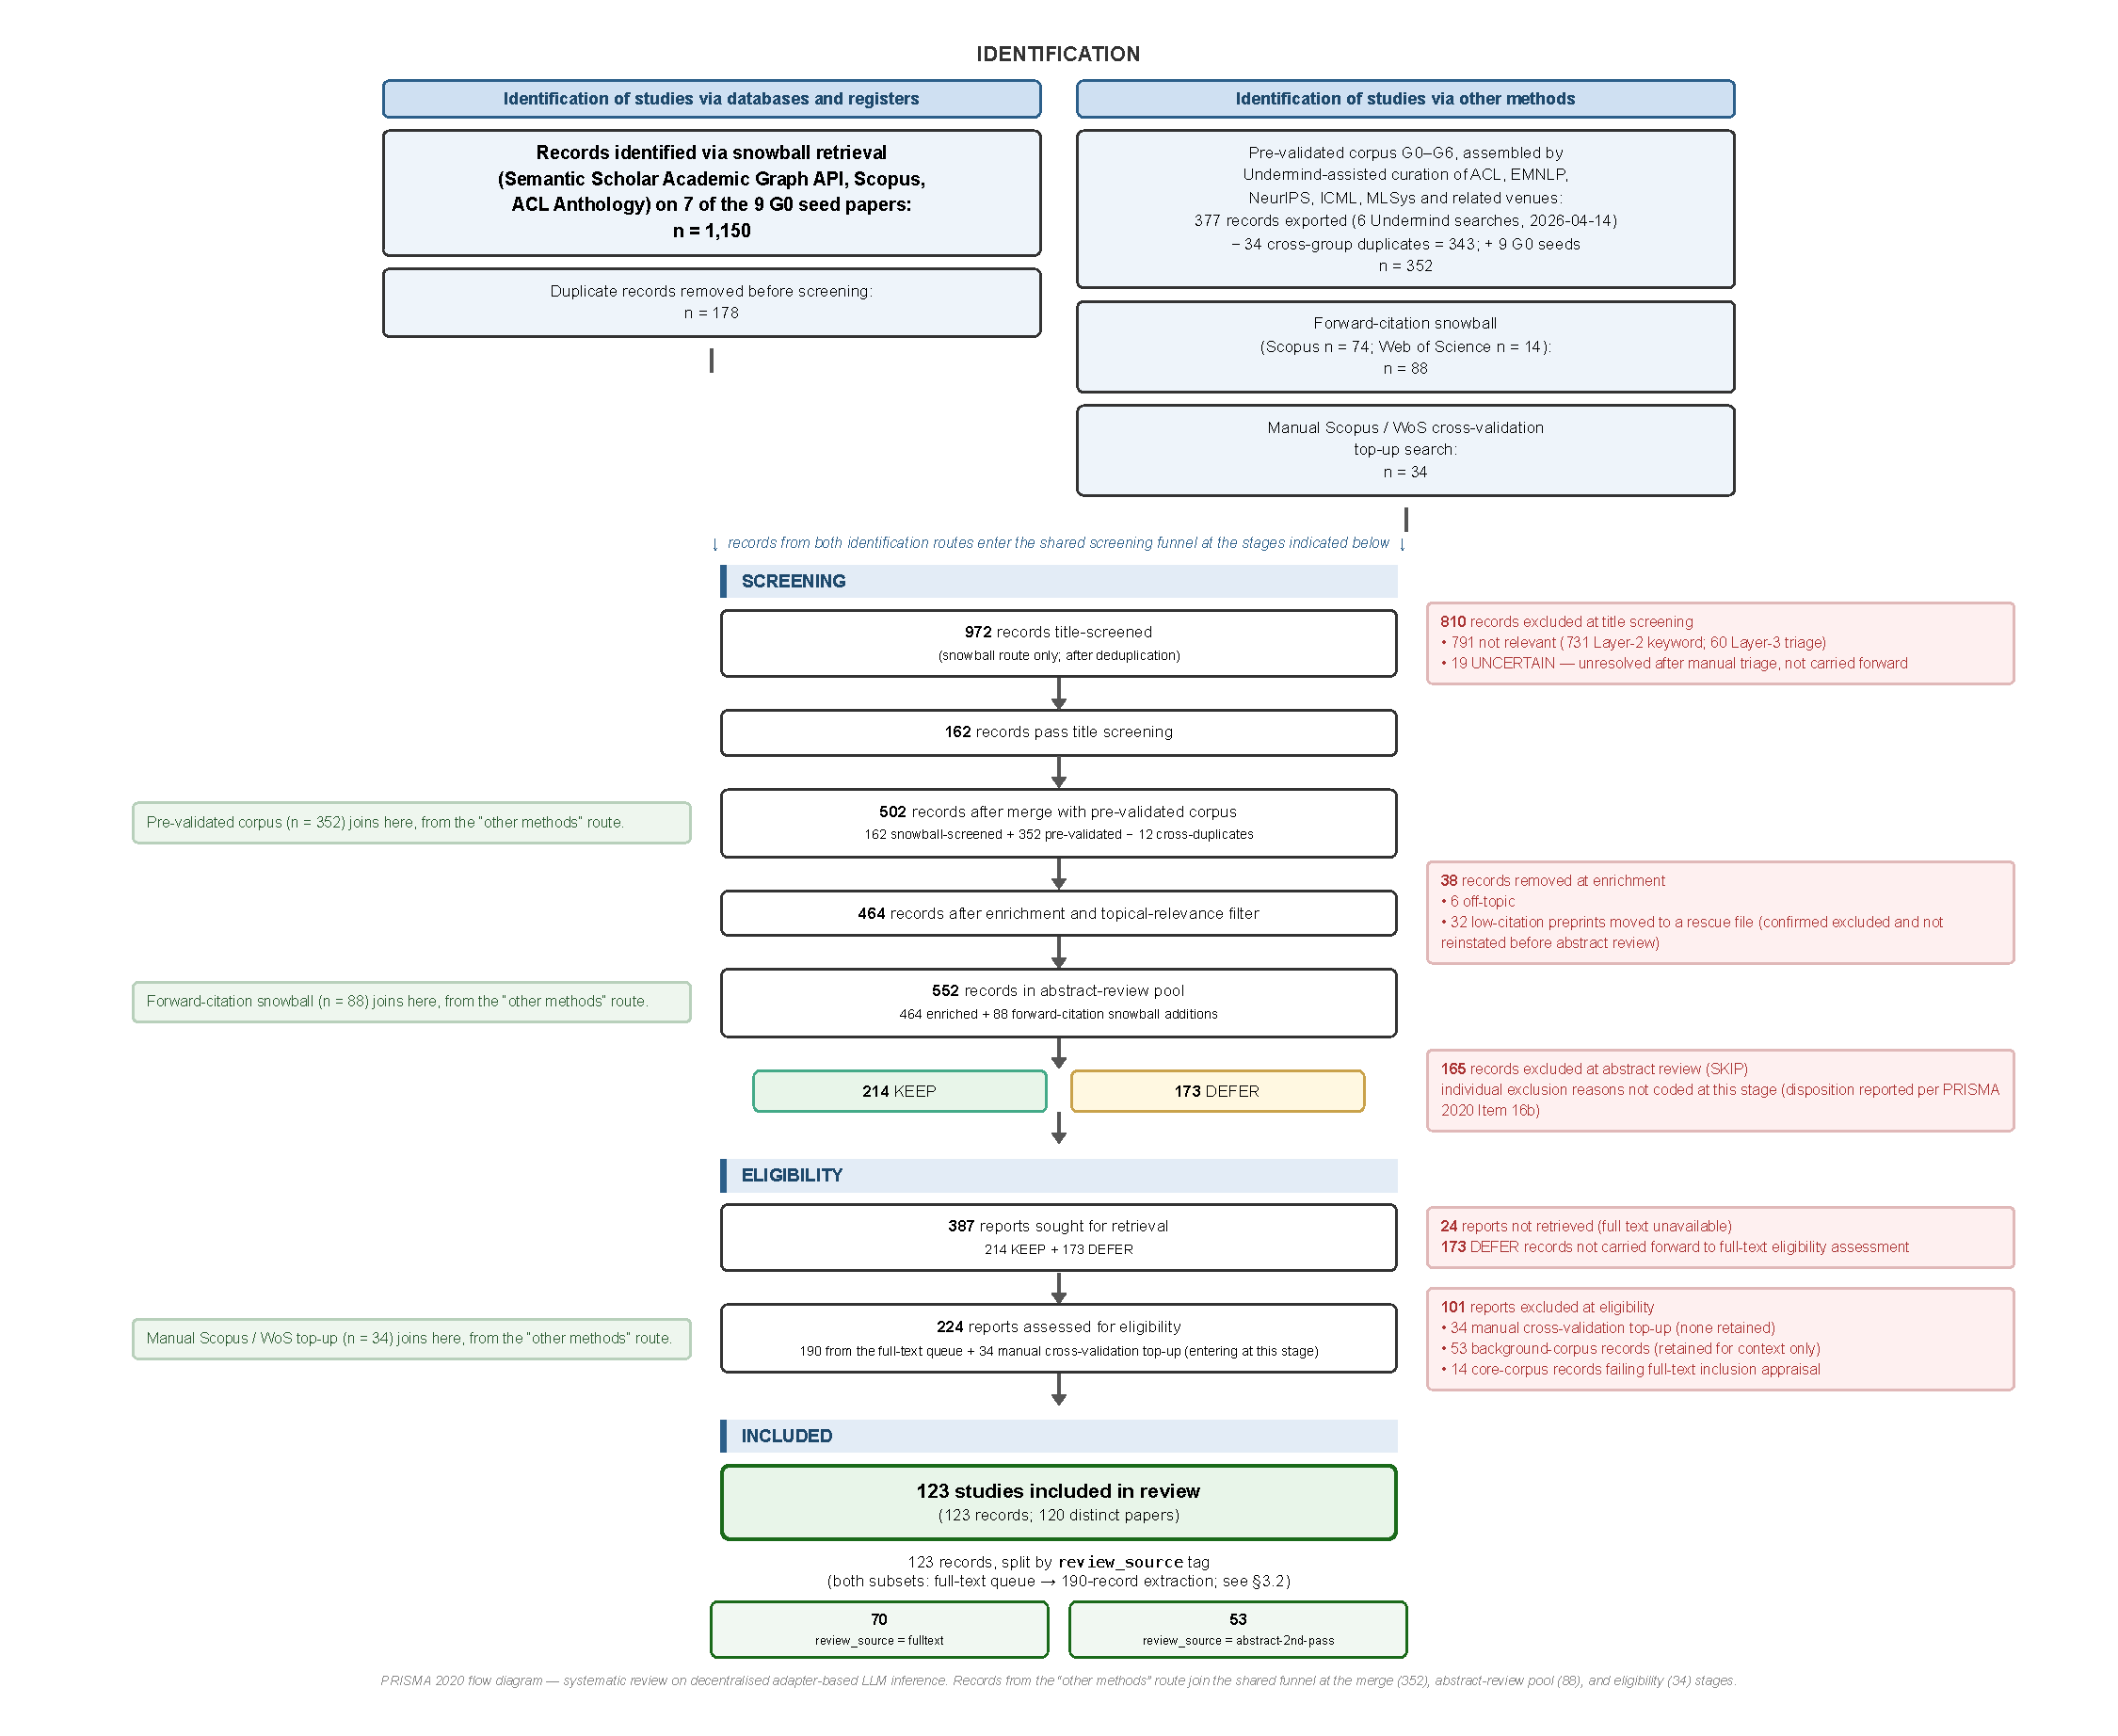
\includegraphics[width=\linewidth]{figures/fig_slr1_prisma_flow.pdf}
  \caption{PRISMA 2020 flow diagram for the systematic literature review.
           Records trace from 1,150 raw snowball candidates through deduplication,
           title screening, enrichment, abstract review, and full-text assessment to
           the 123-paper final reading list.}
  \label{fig:prisma}
\end{figure}

\subsection{Datasets and Benchmarks}
\label{sec:methodology:datasets}

Table~\ref{tab:datasets} presents the datasets, task types, and evaluation
metrics reported by each of the 18 representative systems from the concept
matrix (Table~\ref{tab:concept_matrix} in Section~\ref{sec:synthesis_gap:matrix}), supplemented with closely related
PEFT and composition baselines. The data were extracted from the full-text
reading of each paper (see Appendix~B for extraction notes). PEFT papers
predominantly evaluate on GLUE \citep{WangGLUE2018}, SuperGLUE \citep{WangSuperGLUE2019}, and MMLU \citep{HendrycksMMLU2021}; serving papers rely on
synthetic throughput benchmarks. Notably, no single benchmark spans all three 
pillars simultaneously: PEFT papers evaluate on GLUE and SuperGLUE, serving papers 
rely on synthetic throughput workloads, and federated PEFT papers introduce 
privacy-oriented datasets. This fragmentation limits direct cross-pillar 
comparison and is reflected in the empirical gaps discussed in Section~\ref{sec:synthesis_gap}.


\begin{sidewaystable}[p]
\centering
\caption{Selected datasets, tasks, and metrics. Full corpus: Appendix~B.}
\label{tab:datasets}
\small
\setlength{\tabcolsep}{5pt}
  \resizebox{\textwidth}{!}{%
  \begin{tabular}{lllllc}
  \toprule
  \textbf{Paper} & \textbf{Dataset} & \textbf{Task Type} & \textbf{Metric} &
  \textbf{Score} & \textbf{Public} \\
  \midrule
  \multicolumn{6}{l}{\textbf{Pillar 1: PEFT and Adapters}} \\
  Houlsby et al.~\citep{Houlsby2019} & GLUE, SciTail & NLU classification &
  Accuracy & 91.1 (SciTail) & Yes \\
  Hu et al.~\citep{Hu2022} (LoRA) & GLUE & NLU classification & Accuracy & 87.8
  (GLUE avg.) & Yes \\
  Dettmers et al.~\citep{Dettmers2023} (QLoRA) & Vicuna benchmark & instruction
  following & Elo rating & 99.3\% of ChatGPT & Yes \\
  Li~\&~Liang~\citep{LiLiang2021} (Prefix) & E2E, WebNLG, XSUM & NLG & ROUGE-L &
   34.9 (XSUM) & Yes \\
  Ben Zaken et al.~\citep{BenZaken2022} (BitFit) & GLUE & NLU classification &
  Accuracy & $\approx$ BERT-base full FT & Yes \\
  Poth et al.~\citep{PothAdapters2023} (Adapters lib.) & GLUE & NLU
  classification & Accuracy & matches full FT & Yes \\
  \midrule
  \multicolumn{6}{l}{\textbf{Pillar 2: Adapter Composition}} \\
  AdapterHub~\citep{Pfeiffer2020hub} & GLUE, XNLI & NLU + cross-lingual &
  Accuracy & multiple tasks & Yes \\
  AdapterFusion~\citep{Pfeiffer2021fusion} & GLUE, SciTail, MRPC & NLU
  classification & Accuracy & 96.6 (SciTail) & Yes \\
  MAD-X~\citep{PfeifferMADX2020} & GLUE (6 langs) & cross-lingual transfer &
  Accuracy & zero-shot transfer & Yes \\
  LoraHub~\citep{Huang2023} & BIG-Bench Hard & few-shot transfer & Accuracy &
  34.7 avg per task (BBH) & Yes \\
  LoraRetriever~\citep{ZhaoLoraRetriever2024} & domain QA, MT-bench & multi-task
   QA & Accuracy/win-rate & matches best single & Yes \\
  Ostapenko et al.~(2024) & GLUE, SuperGLUE & NLU classification & Accuracy &
  --- & No \\
  \midrule
  \multicolumn{6}{l}{\textbf{Pillar 3: Adapter-Aware Inference Serving}} \\
  S-LoRA~\citep{Sheng2024} & synthetic & throughput & req/s & up to 4$\times$
  throughput & No \\
  Punica~\citep{Chen2023Punica} & synthetic serving & throughput & req/s &
  12$\times$ higher throughput & No \\
  CaraServe~\citep{Li2024CaraServe} & synthetic & throughput & req/s &
  1.4$\times$ on average & No \\
  Petals~\citep{Borzunov2023} & multiple & instruction following & Accuracy &
  multiple & Yes \\
  MT-EF~\citep{Sajina2024} & Reddit, StackOverflow, CoNLL-2003, Few-NERD & MTP +
   NER & Test UA (User Acc.) & +11.6\% mean relative gain & Yes \\
  \midrule
  \multicolumn{6}{l}{\textbf{Pillar 4: P2P and Federated Learning}} \\
  FedAvg~\citep{McMahan2017} & CIFAR-10, Shakespeare & image/text classification
   & Accuracy & 10--100$\times$ comm. saving & Yes \\
  FedProx~\citep{Li2020FedProx} & FEMNIST, Sent140 & image/text classification &
   Accuracy & +1--5\% vs FedAvg & Yes \\
  FedPETuning~\citep{ZhangFedPETuning2023} & GLUE & NLU classification &
  Accuracy & $\leq$5\% loss vs central PEFT & Yes \\
  FLoRA~\citep{WangFLoRA2024} & GLUE (few-shot) & NLU classification & Accuracy
  & robust to rank hete. & Yes \\
DP-FedLoRA~\citep{XuDPFedLoRA2025} & MMLU, BBH, CRASS & NLU + reasoning & Accuracy + $(\epsilon,\delta)$ & $\approx$4--5\% loss at $\epsilon=25$ & Yes \\
  SLoRA~\citep{Babakniya2023} & GLUE, SuperGLUE & NLU classification & Accuracy
  & 2$\times$ faster convergence & Yes \\
  Gossip Learning~\citep{HegeduisGossip2019} & synthetic & classification &
  Accuracy & $\approx$ FL quality (20--50\% slower) & Yes \\
  \midrule
  \multicolumn{6}{l}{\textbf{Pillar 5: MoE and Adapter Routing}} \\
  Switch Transformers~\citep{Fedus2022} & C4 pre-training & language modelling &
   Perplexity, speedup & 4$\times$ speedup over T5-XXL & No \\
  Expert Choice~\citep{Zhou2022} & SuperGLUE, WMT & NLU + MT & Accuracy/BLEU &
  +2\% average accuracy & No \\
  DeepSpeed-MoE~\citep{RajbhandariDeepSpeed2022} & GLUE, SuperGLUE & NLU
  classification & Accuracy & 4.5$\times$ speedup, $<$0.5\% loss & No \\
  AdaMix~\citep{WangAdaMix2022} & GLUE, SuperGLUE & NLU classification &
  Accuracy & outperforms single PEFT & Yes \\
  MixLoRA~\citep{LiMixLoRA2024} & GLUE, domain-specific & NLU classification &
  Accuracy & --- & Yes \\
MiLoRA~\citep{ZhangMiLoRA2024} & commonsense reasoning, math reasoning & 
reasoning + instruction following & Accuracy & $>$ single LoRA & Yes \\
  LoRAMoE~\citep{DouLoRAMoE2024} & world knowledge + instruct & multi-task
  generation & Accuracy, forgetting & alleviates forgetting & No \\
  MOELoRA~\citep{LiuMOELoRA2023} & medical + GLUE & NLU classification &
  Accuracy & $>$ single LoRA & Yes \\
  Crowdsourced MoE~\citep{RyabininCrowdsourced2020} & CIFAR-10/100, MNIST &
  image classification & Accuracy & up to 16 peers, 30\% dropout & No \\
  \midrule
\bottomrule
  \end{tabular}
  }
  \end{sidewaystable}



\subsection{AI Tool Transparency}
\label{sec:methodology:ai}

Two AI-assisted tools were used during the corpus construction pipeline
in a supporting capacity. Their roles and scope are documented here for
reproducibility.

\textbf{Undermind} (undermind.ai) was used to accelerate the retrieval
of candidate papers for Groups G1--G6. For each group, a detailed
research prompt specifying the thematic scope, key seed papers, and
target venues was submitted to Undermind, which returned ranked lists
of candidate papers from ACL, EMNLP, NeurIPS, ICML, MLSys, and related
databases. The six prompts are reproduced verbatim in Appendix~A.
Undermind was used exclusively for \textit{retrieval}, not
\textit{selection}: every returned candidate was reviewed manually by
the author, and inclusion decisions were made independently of
Undermind's ranking.

At the title screening and abstract review stages, the author used an automated
advisory tool (\textbf{Claude AI}, Anthropic) to generate consistency aids.
At the title screening stage, the tool generated preliminary sorting suggestions
for 130 ambiguous records based on title and venue name alone
(Section~\ref{sec:methodology:screening}). At the abstract review stage, it
provided a one-sentence summary and a preliminary relevance recommendation for
each of the 552 records reviewed (Section~\ref{sec:methodology:abstract}). In
both cases, the outputs were strictly advisory: all inclusion and exclusion
decisions were made by the author after independent assessment. Model identifiers,
per-record suggestions, and the author's final decisions are logged in the
screening audit files to support reproducibility.

In addition to the roles described above, AI-assisted tools were used
during manuscript preparation for language editing, structural feedback,
and translation support; all analytical content, literature
interpretation, and final wording remain the author's own.


